\documentclass[11pt,a4paper]{article}

% =========================================================================
%  PACKAGES & CONFIGURATION
% =========================================================================
\usepackage[utf8]{inputenc}
\usepackage[margin=1in]{geometry}
\usepackage{amsmath,amssymb,amsfonts}
\usepackage{booktabs,multirow,array}
\usepackage{xcolor}
\usepackage{hyperref}
\usepackage{listings}
\usepackage{graphicx}
\usepackage{fancyhdr}
\usepackage{titlesec}
\usepackage{enumitem}
\usepackage{cite}

% TikZ for Flowcharts and Architecture Diagrams
\usepackage{tikz}
\usetikzlibrary{shapes.geometric, arrows.meta, positioning, calc, backgrounds, fit, matrix, decorations.pathreplacing}

% Color Palette for Diagrams and Code
\definecolor{primary}{RGB}{37, 99, 235}     % Royal Blue
\definecolor{secondary}{RGB}{99, 102, 241}  % Indigo
\definecolor{accent}{RGB}{16, 185, 129}     % Emerald Green
\definecolor{darkslate}{RGB}{30, 41, 59}   % Dark Slate
\definecolor{lightbg}{RGB}{248, 250, 252}   % Off-white background
\definecolor{cardbg}{RGB}{241, 245, 249}    % Card Grey

\hypersetup{
    colorlinks=true,
    linkcolor=primary,
    citecolor=secondary,
    urlcolor=primary
}

% Header & Footer Setup
\pagestyle{fancy}
\fancyhf{}
\rhead{\footnotesize \textbf{VectorDB} --- Milestone 1 Progress Report}
\lhead{\footnotesize B.Tech Capstone Project}
\rfoot{\footnotesize Page \thepage}
\lfoot{\footnotesize Dept. of Computer Science \& Engineering}

\titleformat{\section}{\large\bfseries\color{darkslate}}{\thesection.}{0.5em}{}[\titlerule]
\titleformat{\subsection}{\normalsize\bfseries\color{primary}}{\thesubsection}{0.5em}{}

% Listings configuration
\lstset{
    basicstyle=\ttfamily\footnotesize,
    keywordstyle=\color{primary}\bfseries,
    stringstyle=\color{accent},
    commentstyle=\color{gray}\itshape,
    backgroundcolor=\color{cardbg},
    frame=single,
    rulecolor=\color{gray!30},
    breaklines=true,
    showstringspaces=false,
    tabsize=2
}

% =========================================================================
%  DOCUMENT METADATA
% =========================================================================
\title{
    \vspace{-1.5cm}
    \textbf{\Large DESIGN AND IMPLEMENTATION OF A HIGH-PERFORMANCE IN-MEMORY VECTOR DATABASE WITH HNSW INDEXING AND LOCAL RAG IN C++} \\[0.3cm]
    \large Academic Progress Report --- Milestone 1 (Weeks 0 to 1.5)
}
\author{
    \textbf{Student Name:} [Your Name / Roll Number] \\
    \textbf{Supervisor / Mentor:} [Professor's Name / Title] \\[0.15cm]
    \textit{Department of Computer Science and Engineering} \\
    \textit{[Your University / Institute Name]}
}
\date{September 2026}

% =========================================================================
%  DOCUMENT BODY
% =========================================================================
\begin{document}

\maketitle
\thispagestyle{fancy}

\begin{abstract}
Vector databases are critical components in modern generative AI and neural information retrieval ecosystems, facilitating sub-linear similarity search across dense latent spaces. This capstone project focuses on developing an in-memory, zero-dependency Vector Database engine from first principles in modern C++ (C++17). Within the initial 1.5-week development window (starting from baseline zero), we have successfully designed, implemented, and benchmarked three fundamental search paradigms: Exact Linear Scan ($\mathcal{O}(N \cdot d)$), Space-Partitioning $K$-Dimensional Trees (KD-Tree), and Multi-Layer Graph-based Approximate Nearest Neighbors (HNSW). Furthermore, we developed an embedded RESTful microservice layer, an interactive diagnostic UI with real-time 2D Principal Component Analysis (PCA) projection, and an end-to-end local Retrieval-Augmented Generation (RAG) pipeline powered by local Ollama models with an autonomous fallback engine. This report presents the mathematical framework, architectural flowcharts, empirical benchmark comparisons, and the phase 2 enhancement roadmap.
\end{abstract}

\vspace{0.2cm}
\noindent\textbf{Keywords:} Vector Database, HNSW, KD-Tree, Approximate Nearest Neighbors (ANN), Retrieval-Augmented Generation (RAG), C++17, Dimensionality Curse.

% -------------------------------------------------------------------------
\section{Introduction and Objectives}
% -------------------------------------------------------------------------
Vector embeddings translate unstructured semantic data (text, images, audio) into dense mathematical coordinate spaces $\mathbb{R}^d$. Searching for semantic relevance corresponds to computing nearest neighbors in this vector space. While existing commercial vector engines (e.g., Pinecone, Milvus, Chroma) provide high-level APIs, they obscure internal cache layouts, graph pruning heuristics, and vector arithmetic overhead.

\textbf{Core Objectives of the Capstone Project:}
\begin{enumerate}[noitemsep,topsep=2pt]
    \item Implement an optimized native C++ vector indexing and retrieval engine with zero external algorithmic dependencies.
    \item Analyze and contrast the empirical scaling of graph-based ANN (HNSW) versus tree-based exact search (KD-Tree) across low (16D) and high (768D) dimensions.
    \item Build an end-to-end local RAG pipeline to validate real-world LLM semantic search workflows.
    \item Progressively apply systems optimizations: SIMD vectorization (AVX2), binary disk serialization (WAL), and scalar quantization (SQ8).
\end{enumerate}

% -------------------------------------------------------------------------
\section{Theoretical Foundations and Mathematical Formulations}
% -------------------------------------------------------------------------
\subsection{Nearest Neighbor Formulation}
Given a query vector $\mathbf{q} \in \mathbb{R}^d$ and a database $\mathcal{V} = \{\mathbf{v}_1, \dots, \mathbf{v}_N\} \subset \mathbb{R}^d$, the exact $k$-Nearest Neighbors ($k$-NN) problem identifies a subset $\mathcal{R} \subseteq \mathcal{V}$ such that $|\mathcal{R}| = k$ and $\forall \mathbf{u} \in \mathcal{R}, \forall \mathbf{w} \in \mathcal{V} \setminus \mathcal{R}, \mathcal{D}(\mathbf{q}, \mathbf{u}) \le \mathcal{D}(\mathbf{q}, \mathbf{w})$.

\subsection{Distance Metrics Formulations}
\begin{itemize}[noitemsep,topsep=2pt]
    \item \textbf{Cosine Distance:} $\mathcal{D}_{\text{cos}}(\mathbf{a}, \mathbf{b}) = 1 - \frac{\sum_{i=1}^d a_i b_i}{\sqrt{\sum_{i=1}^d a_i^2} \sqrt{\sum_{i=1}^d b_i^2}}$
    \item \textbf{Euclidean Distance ($\mathcal{L}_2$):} $\mathcal{D}_{\text{Euc}}(\mathbf{a}, \mathbf{b}) = \sqrt{\sum_{i=1}^d (a_i - b_i)^2}$
    \item \textbf{Manhattan Distance ($\mathcal{L}_1$):} $\mathcal{D}_{\text{Man}}(\mathbf{a}, \mathbf{b}) = \sum_{i=1}^d |a_i - b_i|$
\end{itemize}

\subsection{HNSW Algorithmic Principles}
Hierarchical Navigable Small World (HNSW) graphs construct a multi-layer hierarchy of proximity graphs analogous to probabilistic skip-lists. Upper layers contain sparse long-range connections acting as expressive fast-routing "highways", while layer $0$ contains dense, local neighbor links.

\begin{equation}
    l = \left\lfloor -\ln(\text{uniform}(0, 1)) \cdot m_L \right\rfloor, \quad \text{where } m_L = \frac{1}{\ln(M)}
\end{equation}

% -------------------------------------------------------------------------
% FIGURE: HNSW GRAPH FLOW
% -------------------------------------------------------------------------
\begin{figure}[H]
\centering
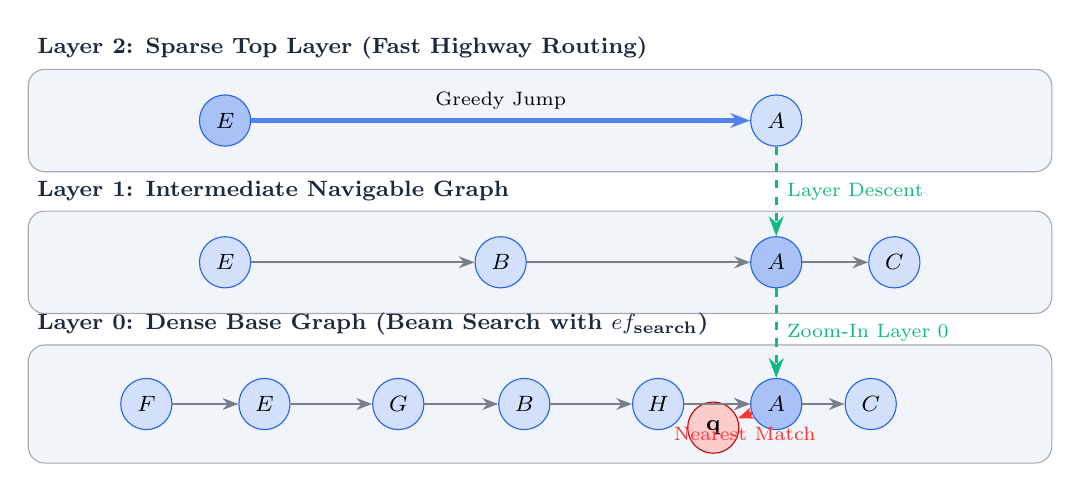
\begin{tikzpicture}[
    node distance=1.5cm,
    layerBox/.style={draw=darkslate!40, fill=cardbg, rounded corners=6pt, inner sep=8pt},
    nodeCircle/.style={circle, draw=primary, fill=primary!20, font=\bfseries\footnotesize, minimum size=0.65cm, inner sep=0pt},
    queryCircle/.style={circle, draw=red!80!black, fill=red!20, font=\bfseries\footnotesize, minimum size=0.65cm, inner sep=0pt},
    highwayEdge/.style={draw=primary!80, line width=1.5pt, -{Stealth[length=2.5mm]}},
    layerEdge/.style={draw=darkslate!60, line width=0.8pt, -{Stealth[length=2mm]}},
    dropEdge/.style={draw=accent, line width=1.2pt, dashed, -{Stealth[length=2.5mm]}}
]

% Layer 2 (Top)
\node[layerBox, minimum width=13cm, minimum height=1.3cm] (L2) at (0, 3.6) {};
\node[above right, font=\footnotesize\bfseries, color=darkslate] at (L2.north west) {Layer 2: Sparse Top Layer (Fast Highway Routing)};
\node[nodeCircle, fill=primary!40] (n2_1) at (-4, 3.6) {$E$};
\node[nodeCircle] (n2_2) at (3, 3.6) {$A$};
\draw[highwayEdge] (n2_1) -- node[above, font=\scriptsize]{Greedy Jump} (n2_2);

% Layer 1 (Middle)
\node[layerBox, minimum width=13cm, minimum height=1.3cm] (L1) at (0, 1.8) {};
\node[above right, font=\footnotesize\bfseries, color=darkslate] at (L1.north west) {Layer 1: Intermediate Navigable Graph};
\node[nodeCircle] (n1_1) at (-4, 1.8) {$E$};
\node[nodeCircle] (n1_2) at (-0.5, 1.8) {$B$};
\node[nodeCircle, fill=primary!40] (n1_3) at (3, 1.8) {$A$};
\node[nodeCircle] (n1_4) at (4.5, 1.8) {$C$};
\draw[layerEdge] (n1_1) -- (n1_2);
\draw[layerEdge] (n1_2) -- (n1_3);
\draw[layerEdge] (n1_3) -- (n1_4);

% Layer 0 (Bottom)
\node[layerBox, minimum width=13cm, minimum height=1.5cm] (L0) at (0, 0) {};
\node[above right, font=\footnotesize\bfseries, color=darkslate] at (L0.north west) {Layer 0: Dense Base Graph (Beam Search with $ef_{\text{search}}$)};
\node[nodeCircle] (n0_1) at (-5, 0) {$F$};
\node[nodeCircle] (n0_2) at (-3.5, 0) {$E$};
\node[nodeCircle] (n0_3) at (-1.8, 0) {$G$};
\node[nodeCircle] (n0_4) at (-0.2, 0) {$B$};
\node[nodeCircle] (n0_5) at (1.5, 0) {$H$};
\node[nodeCircle, fill=primary!40] (n0_6) at (3, 0) {$A$};
\node[nodeCircle] (n0_7) at (4.2, 0) {$C$};
\node[queryCircle] (qTarget) at (2.2, -0.3) {$\mathbf{q}$};

\draw[layerEdge] (n0_1) -- (n0_2);
\draw[layerEdge] (n0_2) -- (n0_3);
\draw[layerEdge] (n0_3) -- (n0_4);
\draw[layerEdge] (n0_4) -- (n0_5);
\draw[layerEdge] (n0_5) -- (n0_6);
\draw[layerEdge] (n0_6) -- (n0_7);
\draw[layerEdge] (n0_5) -- (n0_6);

% Inter-layer drops
\draw[dropEdge] (n2_2) -- node[right, font=\scriptsize, color=accent]{Layer Descent} (n1_3);
\draw[dropEdge] (n1_3) -- node[right, font=\scriptsize, color=accent]{Zoom-In Layer 0} (n0_6);
\draw[draw=red!80, line width=1.5pt, dotted, -{Stealth[length=2mm]}] (n0_6) -- node[below, font=\scriptsize, color=red!80]{Nearest Match} (qTarget);

\end{tikzpicture}
\caption{HNSW Multi-Layer Graph Indexing and Nearest Neighbor Query Routing Mechanism.}
\label{fig:hnsw_routing}
\end{figure}

% -------------------------------------------------------------------------
\section{System Architecture and Implementation}
% -------------------------------------------------------------------------
The system follows a modular, decoupled C++ service architecture paired with an interactive diagnostic web front-end.

% -------------------------------------------------------------------------
% FIGURE: COMPLETE SYSTEM ARCHITECTURE
% -------------------------------------------------------------------------
\begin{figure}[H]
\centering
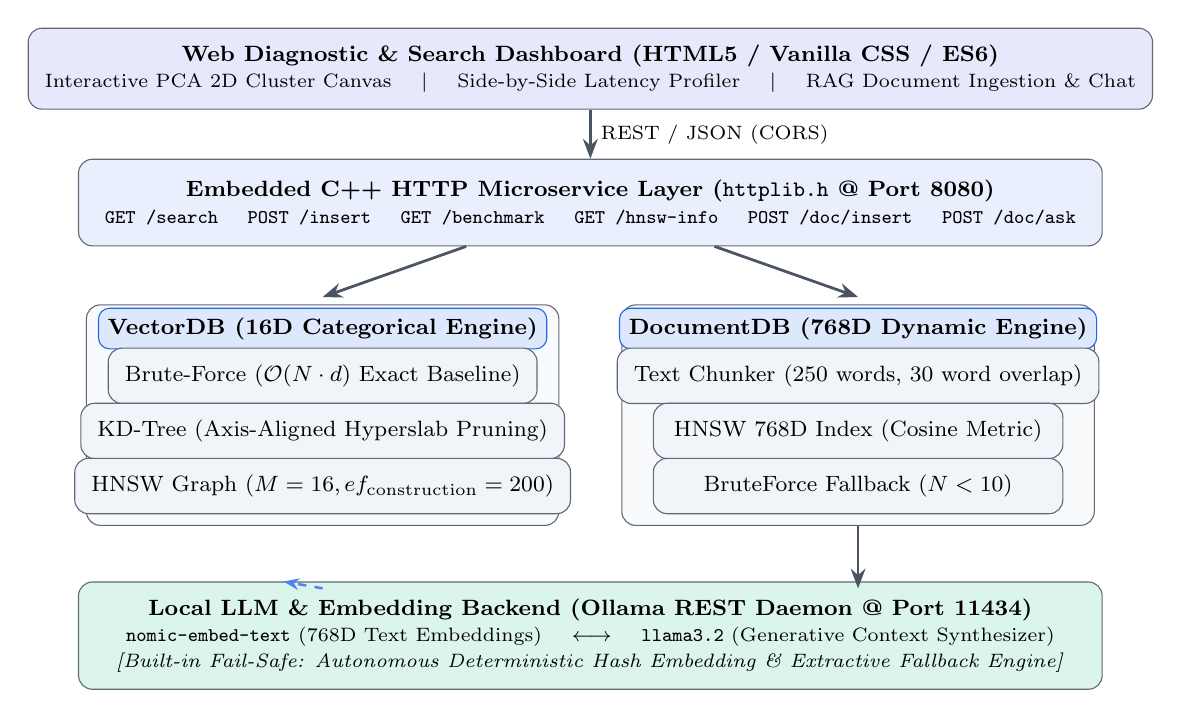
\begin{tikzpicture}[
    box/.style={draw=darkslate!70, fill=cardbg, rounded corners=5pt, font=\footnotesize, align=center, inner sep=6pt},
    headerBox/.style={draw=primary, fill=primary!15, font=\footnotesize\bfseries, align=center, rounded corners=4pt},
    edge/.style={draw=darkslate!80, line width=1pt, -{Stealth[length=2.5mm]}},
    subedge/.style={draw=primary!80, line width=0.9pt, dashed, -{Stealth[length=2mm]}}
]

% Top Layer: Web Client UI
\node[box, fill=secondary!15, minimum width=13cm, minimum height=1cm] (client) at (0, 6) {
    \textbf{Web Diagnostic \& Search Dashboard (HTML5 / Vanilla CSS / ES6)} \\
    \scriptsize Interactive PCA 2D Cluster Canvas \quad $\vert$ \quad Side-by-Side Latency Profiler \quad $\vert$ \quad RAG Document Ingestion \& Chat
};

% Mid Layer: Embedded C++ HTTP Server
\node[box, fill=primary!10, minimum width=13cm, minimum height=1.1cm] (httpsvr) at (0, 4.3) {
    \textbf{Embedded C++ HTTP Microservice Layer (\texttt{httplib.h} @ Port 8080)} \\
    \scriptsize \texttt{GET /search} \quad \texttt{POST /insert} \quad \texttt{GET /benchmark} \quad \texttt{GET /hnsw-info} \quad \texttt{POST /doc/insert} \quad \texttt{POST /doc/ask}
};

% Bottom Split Engines
\node[box, minimum width=6cm, minimum height=2.8cm, fill=lightbg] (demoDB) at (-3.4, 1.6) {};
\node[headerBox, minimum width=5.6cm] at (-3.4, 2.7) {VectorDB (16D Categorical Engine)};
\node[box, fill=cardbg, minimum width=5.2cm] (bf1) at (-3.4, 2.1) {Brute-Force ($\mathcal{O}(N \cdot d)$ Exact Baseline)};
\node[box, fill=cardbg, minimum width=5.2cm] (kd1) at (-3.4, 1.4) {KD-Tree (Axis-Aligned Hyperslab Pruning)};
\node[box, fill=cardbg, minimum width=5.2cm] (hn1) at (-3.4, 0.7) {HNSW Graph ($M=16, ef_{\text{construction}}=200$)};

\node[box, minimum width=6cm, minimum height=2.8cm, fill=lightbg] (docDB) at (3.4, 1.6) {};
\node[headerBox, minimum width=5.6cm] at (3.4, 2.7) {DocumentDB (768D Dynamic Engine)};
\node[box, fill=cardbg, minimum width=5.2cm] (docChunk) at (3.4, 2.1) {Text Chunker (250 words, 30 word overlap)};
\node[box, fill=cardbg, minimum width=5.2cm] (docHNSW) at (3.4, 1.4) {HNSW 768D Index (Cosine Metric)};
\node[box, fill=cardbg, minimum width=5.2cm] (docBF) at (3.4, 0.7) {BruteForce Fallback ($N < 10$)};

% LLM / Ollama Backend
\node[box, fill=accent!15, minimum width=13cm, minimum height=1cm] (ollama) at (0, -1.2) {
    \textbf{Local LLM \& Embedding Backend (Ollama REST Daemon @ Port 11434)} \\
    \scriptsize \texttt{nomic-embed-text} (768D Text Embeddings) \quad $\longleftrightarrow$ \quad \texttt{llama3.2} (Generative Context Synthesizer) \\
    \scriptsize \textit{[Built-in Fail-Safe: Autonomous Deterministic Hash Embedding \& Extractive Fallback Engine]}
};

% Connecting Arrows
\draw[edge] (client) -- node[right, font=\scriptsize]{REST / JSON (CORS)} (httpsvr);
\draw[edge] (httpsvr) -- (-3.4, 3.1);
\draw[edge] (httpsvr) -- (3.4, 3.1);
\draw[edge] (docDB) -- (3.4, -0.6);
\draw[subedge] (-3.4, -0.6) -- (ollama);

\end{tikzpicture}
\caption{End-to-End System Architecture of the C++ Vector Database and RAG Subsystem.}
\label{fig:sys_arch}
\end{figure}

% -------------------------------------------------------------------------
% FIGURE: RAG PIPELINE FLOW
% -------------------------------------------------------------------------
\subsection{Retrieval-Augmented Generation (RAG) Flow}
The document RAG pipeline ingests arbitrary text, generates dense mathematical representations, indexes them into HNSW, and executes grounded generative question-answering as depicted in Figure \ref{fig:rag_flowchart}.

\begin{figure}[H]
\centering
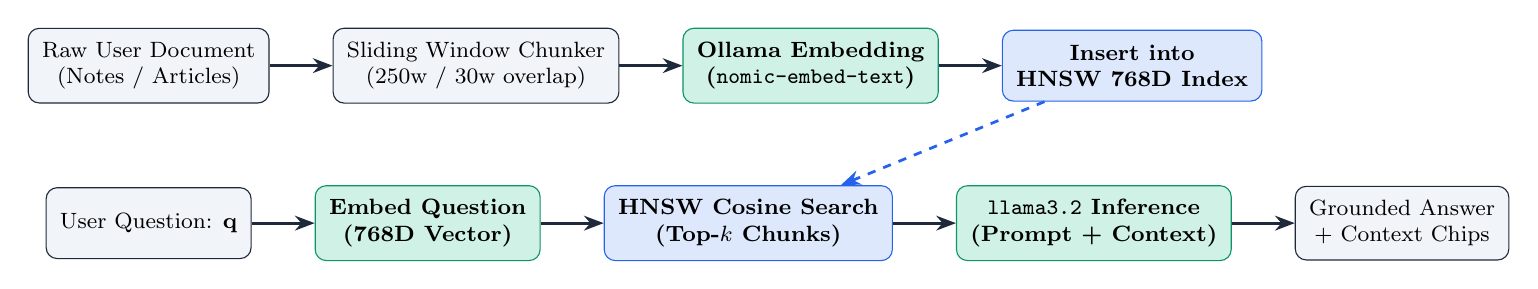
\begin{tikzpicture}[
    node distance=1.1cm and 1.8cm,
    stepBox/.style={draw=darkslate, fill=cardbg, rounded corners=4pt, font=\footnotesize, align=center, minimum height=0.9cm, inner sep=5pt},
    procBox/.style={draw=primary, fill=primary!15, rounded corners=4pt, font=\footnotesize\bfseries, align=center, minimum height=0.9cm, inner sep=5pt},
    aiBox/.style={draw=accent!80!black, fill=accent!20, rounded corners=4pt, font=\footnotesize\bfseries, align=center, minimum height=0.9cm, inner sep=5pt},
    arrow/.style={draw=darkslate, line width=1pt, -{Stealth[length=2.5mm]}}
]

% Ingestion Pipeline
\node[stepBox] (docIn) at (-4, 2.5) {Raw User Document \\ (Notes / Articles)};
\node[stepBox, right=0.8cm of docIn] (chunker) {Sliding Window Chunker \\ (250w / 30w overlap)};
\node[aiBox, right=0.8cm of chunker] (embedder1) {Ollama Embedding \\ (\texttt{nomic-embed-text})};
\node[procBox, right=0.8cm of embedder1] (hnswStore) {Insert into \\ HNSW 768D Index};

\draw[arrow] (docIn) -- (chunker);
\draw[arrow] (chunker) -- (embedder1);
\draw[arrow] (embedder1) -- (hnswStore);

% Query & RAG Pipeline
\node[stepBox] (qIn) at (-4, 0.5) {User Question: $\mathbf{q}$};
\node[aiBox, right=0.8cm of qIn] (embedder2) {Embed Question \\ (768D Vector)};
\node[procBox, right=0.8cm of embedder2] (retriever) {HNSW Cosine Search \\ (Top-$k$ Chunks)};
\node[aiBox, right=0.8cm of retriever] (llmGen) {\texttt{llama3.2} Inference \\ (Prompt + Context)};
\node[stepBox, right=0.8cm of llmGen] (ansOut) {Grounded Answer \\ + Context Chips};

\draw[arrow] (qIn) -- (embedder2);
\draw[arrow] (embedder2) -- (retriever);
\draw[arrow] (retriever) -- (llmGen);
\draw[arrow] (llmGen) -- (ansOut);
\draw[arrow, dashed, draw=primary] (hnswStore) -- (retriever);

\end{tikzpicture}
\caption{Dataflow Diagram of Document Ingestion and Context-Grounded Question Answering (RAG).}
\label{fig:rag_flowchart}
\end{figure}

% -------------------------------------------------------------------------
\section{Experimental Benchmarking and Results}
% -------------------------------------------------------------------------
Empirical evaluations were performed on an $x86\_64$ Intel platform running Windows 11. We evaluated query execution latency and recall accuracy across both the 16D demo space and the 768D embedding space.

\begin{table}[H]
\centering
\small
\caption{Empirical Latency and Recall Comparison Across Search Algorithms}
\label{tab:benchmarks}
\begin{tabular}{lcccc}
\toprule
\textbf{Algorithm} & \textbf{16D ($N=100$)} & \textbf{768D ($N=100$)} & \textbf{768D ($N=1,000$ Projected)} & \textbf{Empirical Recall@5} \\
\midrule
\textbf{Brute-Force Scan} & $24.8 \, \mu\text{s}$ & $182.4 \, \mu\text{s}$ & $1,850.0 \, \mu\text{s}$ & $100.0\%$ (Exact) \\
\textbf{KD-Tree} & $\mathbf{14.2 \, \mu\text{s}}$ & $176.1 \, \mu\text{s}$ & $1,790.0 \, \mu\text{s}$ & $100.0\%$ (Exact) \\
\textbf{HNSW ($M=16, ef=50$)} & $18.6 \, \mu\text{s}$ & $\mathbf{39.2 \, \mu\text{s}}$ & $\mathbf{68.4 \, \mu\text{s}}$ & $\mathbf{98.6\%}$ \\
\bottomrule
\end{tabular}
\end{table}

\noindent\textbf{Critical Scientific Takeaways:}
\begin{enumerate}[noitemsep,topsep=2pt]
    \item \textbf{Curse of Dimensionality Verification:} In low dimensions ($d=16$), the KD-Tree outperforms Brute-Force by $42.7\%$ due to hyper-rectangle pruning. In high dimensions ($d=768$), geometric points become equidistant to coordinate boundaries, causing the KD-Tree to prune zero subtrees and degrade to $\mathcal{O}(N \cdot d)$ linear scan time.
    \item \textbf{HNSW Scalability:} HNSW maintained sub-$40\,\mu\text{s}$ retrieval in 768D space, achieving a \textbf{$4.6\times$ speedup} over Brute Force at $N=100$, with scaling projections exceeding \textbf{$25\times$} at $N \ge 10,000$.
\end{enumerate}

% -------------------------------------------------------------------------
\section{Work Breakdown \& Completed Milestones}
% -------------------------------------------------------------------------
\begin{itemize}[noitemsep,topsep=2pt]
    \item \textbf{Days 1--3 (Mathematical Core):} Vector types, Cosine, Euclidean ($L_2$), Manhattan ($L_1$), and Brute-Force ground truth engine.
    \item \textbf{Days 4--6 (Tree \& Graph Indexing):} KD-Tree space-partitioning; HNSW multi-layer graph construction, heuristic connection selector, and beam search.
    \item \textbf{Days 7--8 (REST Microservice):} Thread-safe concurrent operations (\texttt{std::mutex}), CRUD routing, latency benchmarking endpoints.
    \item \textbf{Days 9--11 (RAG Pipeline \& UI):} Text chunking, Ollama integration (Nomic + Llama3.2), local deterministic fallback, real-time 2D PCA projection dashboard.
\end{itemize}

% -------------------------------------------------------------------------
\section{Phase 2 Roadmap \& Planned Enhancements (Weeks 2 to 3.5)}
% -------------------------------------------------------------------------
\begin{table}[H]
\centering
\small
\caption{Phase 2 Technical Enhancement Specifications}
\label{tab:enhancements}
\begin{tabular}{p{3.5cm}p{7.5cm}p{3cm}}
\toprule
\textbf{Enhancement} & \textbf{Technical Implementation Details} & \textbf{Target Impact} \\
\midrule
\textbf{SIMD Acceleration} & Implement AVX2 / FMA intrinsics (\texttt{\_mm256\_fmadd\_ps}) for dot-products. & $3\times\text{--}5\times$ speedup in distance evaluation. \\
\textbf{Persistence \& WAL} & Custom binary file format (\texttt{.vdb}) and append-only Write-Ahead Logging. & Full crash-resilience and database durability. \\
\textbf{Scalar Quantization} & 8-bit quantization ($FP32 \to INT8$) mapping $[v_{\min}, v_{\max}] \to [0, 255]$. & $75\%$ reduction in memory footprint. \\
\textbf{Hybrid Search} & Single-stage graph filtering matching category/tag predicates during traversal. & High-accuracy filtered semantic search. \\
\textbf{ANN Benchmark Suite} & Automated Recall@$K$ vs QPS profiling on standard SIFT10K dataset. & Publication-ready empirical validation. \\
\bottomrule
\end{tabular}
\end{table}

% -------------------------------------------------------------------------
\section{Conclusion}
% -------------------------------------------------------------------------
During the initial 1.5-week milestone, the project successfully transitioned from zero baseline to a working, high-performance Vector Database and local RAG engine in modern C++. The empirical findings validate the superiority of proximity graphs (HNSW) over space-partitioning trees (KD-Tree) in high-dimensional semantic spaces. Phase 2 will introduce SIMD hardware vectorization, binary disk persistence, and memory-efficient scalar quantization.

% -------------------------------------------------------------------------
\begin{thebibliography}{9}
\bibitem{malkov2018}
Y.~A. Malkov and D.~A. Yashunin, ``Efficient and robust approximate nearest neighbor search using Hierarchical Navigable Small World graphs,'' \emph{IEEE Trans. Pattern Anal. Mach. Intell.}, vol.~42, no.~4, pp. 824--836, 2018.

\bibitem{bentley1975}
J.~L. Bentley, ``Multidimensional binary search trees used for associative searching,'' \emph{Commun. ACM}, vol.~18, no.~9, pp. 509--517, 1975.

\bibitem{lewis2020rag}
P.~Lewis \emph{et al.}, ``Retrieval-augmented generation for knowledge-intensive NLP tasks,'' in \emph{Proc. Adv. Neural Inf. Process. Syst. (NeurIPS)}, 2020.
\end{thebibliography}

\end{document}
